\section{Scale Invariant Feature Transform (SIFT) Based Approach}

\subsection{Short Time Fourier Transform}

\begin{figure}[H]
    \centering
    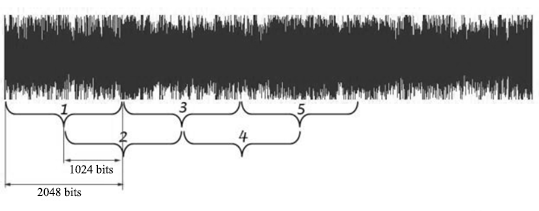
\includegraphics[scale=0.6]{parameters.png}
    \caption{Key parameters on \ac{stft}. 2048 bits long window with 1024 bits long overlapping area.}
    \label{fig:spectrogram_parameters}
  \end{figure}

\subsection{SIFT Descriptor Extraction}

\begin{figure}[H]
    \centering
    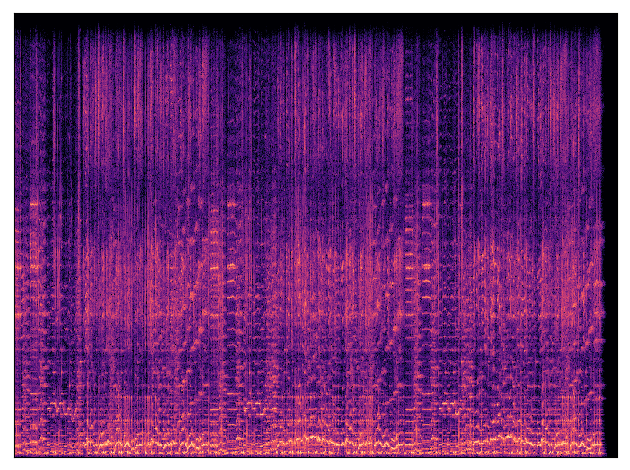
\includegraphics[scale=0.5]{spectrogram.png}
    \caption{Generated colour image of a spectrogram}
    \label{fig:spectrogram_design}
  \end{figure}

  \begin{figure}[H]
    \centering
    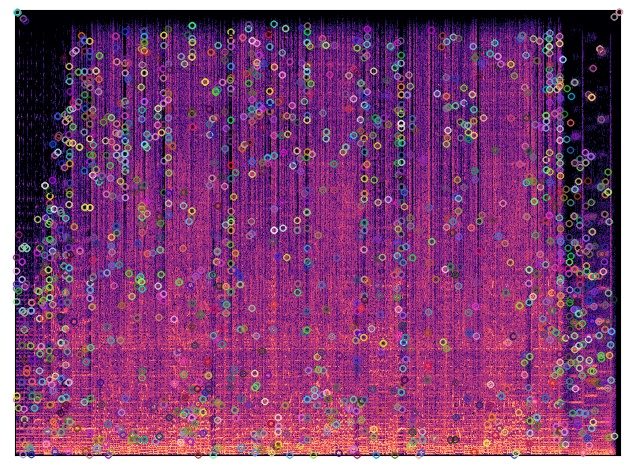
\includegraphics[scale=0.5]{sift_keypoints.jpg}
    \caption{Identified keypoints in a SIFT spectrogram}
    \label{fig:spectrogram_keypoints}
  \end{figure}

\subsection{SIFT Descriptor Matching}

\begin{figure}[H]
    \centering
    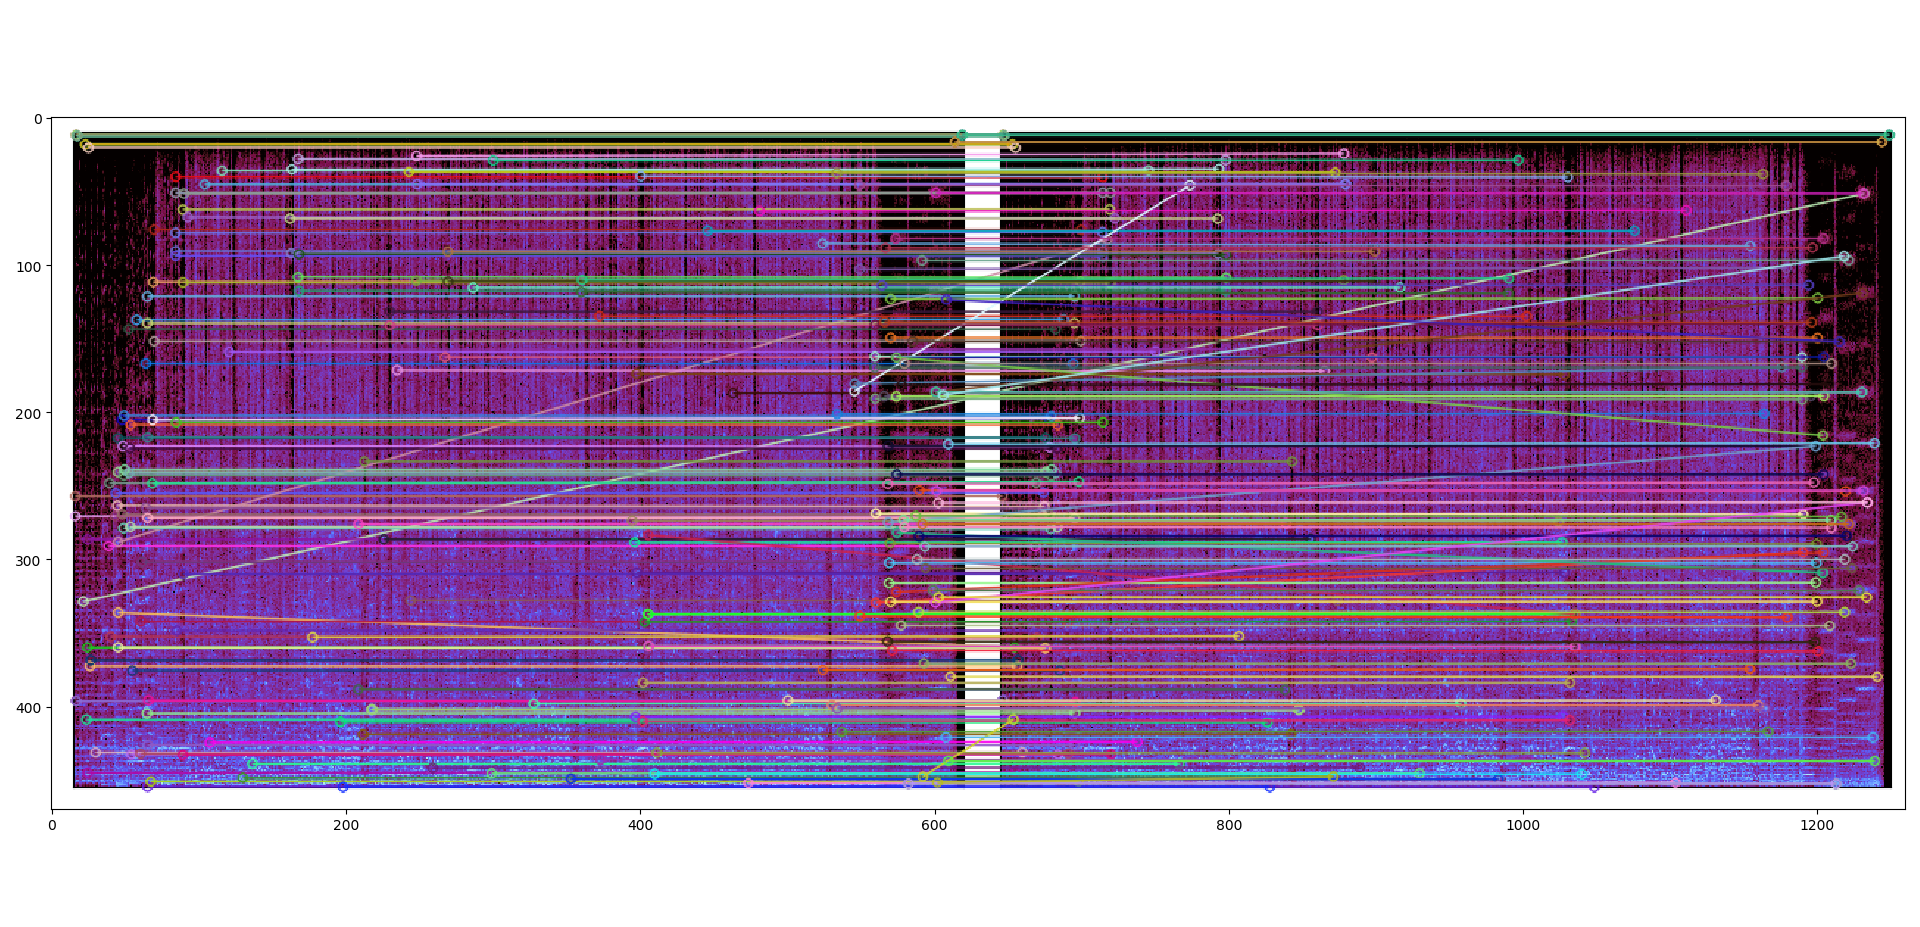
\includegraphics[scale=0.3]{spec_match.png}
    \caption{Matched keypoints of two spectrograms}
    \label{fig:spectrogram_match}
  \end{figure}

\subsection{Thresholding}